\section{Izomeria związków organicznych}

Izomeria- polega na zjawisku, że różne związki chemiczne mające ten sam wzór cząsteczkowy różnią się od siebie sposobem lub kolejnością wiązań chemicznych lub też rozmieszczeniem przestrzennym atomów.
\newline

Izomerię dzielimy na:
\begin{enumerate}
    \item konstytucyjną (strukturalną)- polega na występowaniu związków izomerycznych, w których atomy tych samych pierwiastków są ze sobą połączone w różnej kolejności.
    
    \begin{itemize}
        \item szkieletowa
        
        \begin{itemize}
            \item łańcuchowa- atomy węgla mogą przyjmować różne ułożenia w łańcuchu
            \item pierścieniowa
            \item łańcuchowo- pierścieniowa
        \end{itemize}
        \item podstawienia (położenia) 
        
        \begin{itemize}
            \item położenia podstawnika- różne położenie podstawników w cząsteczce
            \item położenia wiązania wielokrotnego- różne położenie wiązań nienasyconych (wielokrotnych)
        \end{itemize}
        \item funkcyjna- różne podstawniki w cząsteczce (grupy funkcyjne)
    \end{itemize}
    \item stereoizomerię (przestrzenna)- to szczególny rodzaj izomerii, gdzie atomy połączone są między sobą w identycznej kolejności ale różnią się sposobem rozmieszczenia atomów w przestrzeni.
    
    \begin{itemize}
        \item konformacyjna- stereoizomery różniące się między sobą rozmieszczeniem atomów w przestrzeni. Różne konformacje powstają przez obrót poszczególnych części cząsteczki wokół wiązań pojedyńczych i geometrycznie nie przystają do siebie.
        
        \begin{figure}[H]
            \centering
            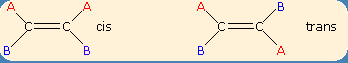
\includegraphics[width=0.7\textwidth]{img/izomer1}
            \label{fig.izomer1}
        \end{figure}
        \item geometryczna- Ten typ izomerii występuje wówczas, gdy w układzie przestrzennym cząsteczki zaznacza się określona płaszczyzna.
        Jeżeli wyróżnione grupy cząsteczki leżą po tej samej stronie płaszczyzny mamy do czynienia z izomerem cis a jeżeli po przeciwnych stronach z izomerem trans.

        \begin{figure}[H]
            \centering
            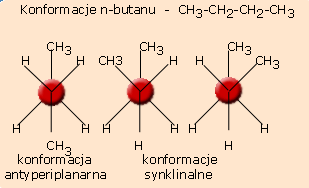
\includegraphics[width=0.7\textwidth]{img/izomery8}
            \label{fig.izomery8}
        \end{figure}
        \item optyczna- Jest to rodzaj stereoizomerii występującej w cząsteczkach chiralnych, które zawierają atom węgla, do którego przyłączone są cztery różne grupy. Taki atom nosi nazwę centrum chiralności.
        A to oznacza, że dla każdej cząsteczki posiadającej centrum chiralności możemy znalezć drugą cząsteczkę będącą jej lustrzanym odbiciem.

        Izomeria optyczna wiąże się ze zdolnością skręcania płaszczyzny światła spolaryzowanego. Substancje takie nazywa się optycznie czynnymi; skręcające płaszczyznę światła spolaryzowanego w prawo - nazywa się prawoskrętnymi /+/, a skręcajace w lewo -lewoskrętnymi /-/.

    \end{itemize}
\end{enumerate}

Izomeria optyczna:
\newline

Izomery bedące wzajemnymi odbiciami lustrzanymi noszą nazwę enacjomerów.

\newpage
Właściwości enancjomerów:
\begin{enumerate}
    \item Enancjomery mają identyczne właściwości fizyczne z wyjątkiem kierunku skręcania płaszczyzny polaryzacji światła
    \item Enancjomery wykazują identyczne właściwości chemiczne; wyjątkiem jest ich zachowanie się w stosunku do optycznie czynnych reagentów. Oznacza to, że jeżeli reagent jest optycznie czynny, jego wpływ na oba enancjomery nie jest identyczny podczas ataku i dlatego szybkość reakcji jest różna - w niektórych przypadkach tak dalece różna, że reakcja z jednym izomerem w ogóle nie zachodzi.
\end{enumerate}

Równocząsteczkowa mieszanina enacjomerów nie wykazuje optycznej czynności i nosi nazwę mieszaniny recemicznej.

Odmiana racemiczna jest optycznie nieczynna. Jest wynikiem równoważenia skręcalności cząsteczki jednego izomeru przez skręcalność cząsteczki drugiego izomeru.
W celu zaznaczenia racemicznego charakteru określonej próbki stosuje się znak (+/-), jak na przykład kwas (+/-)-mlekowy.
\newline

Konfiguracja D- i L-
\newline

Często dla względnego charakteryzowania cząstek chiralnych wprowadzono pojęcie konfiguracji D- i L-, co uwidocznione jest w nazwach związków. Na przykład - aldehyd D-glicerynowy, aldehyd L-glicerynowy

Punktem odniesienia dla konfiguracji D- i L- jest budowa cząsteczki aldehydu glicerynowego a konkretnie położenie podstawników H- oraz HO- przy środkowym węglu.

\begin{figure}[H]
    \centering
    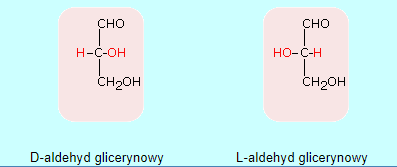
\includegraphics[width=0.7\textwidth]{img/D_L}
    \label{fig.D_L}
\end{figure}

Uporządkowanie na szeregi D i L następuje według konfiguracji podstawników, przy czym bierzemy pod uwagę to centrum chiralności, które jest najbardziej oddalone od grupy karbonylowej.